\documentclass[11pt]{article}
\usepackage[margin=1in]{geometry}
\usepackage[T1]{fontenc}
\usepackage{hyperref}
\usepackage{graphicx}
\usepackage{amsmath}
\usepackage{booktabs}

\title{Waiting is a Choice: Asynchronous Speculative Decoding via Heterogeneous Specialization}
\author{Waiting is a Choice Team}
\date{arXiv preprint, \today}

\begin{document}
\maketitle

\begin{abstract}
Speculative decoding implementations often alternate draft and verify phases with host-visible synchronization points. This can introduce idle gaps that are not fundamental to model math, but to orchestration. We present a reproducible microbenchmark study of a warp-specialized fused kernel that keeps draft and verify work resident on-device. On an RTX 5070 Ti, our final benchmark sweep shows lower latency for fused execution than host-synchronized two-kernel execution. We report this as kernel-level evidence, not an end-to-end LLM serving claim.
\end{abstract}

\section{Introduction}
Deployed speculative decoding systems often follow a draft$\rightarrow$verify rhythm where launch boundaries and host fences shape the visible timeline. We study whether those barriers can be reduced by moving the handoff into one kernel with explicit warp-role partitioning.

\section{Method}
\subsection{Warp specialization}
The fused path (\texttt{k\_fused\_pipeline}) partitions warps into messenger-style draft work and validator-style verify work using shared-memory handoff inside one launch.

\subsection{Cluster and memory path}
The repository includes KV tile prefetch and cluster TMA/DSMEM paths to study overlap and backpressure behavior in a controlled setting.

\subsection{Instrumentation}
Nsight Systems captures use NVTX ranges (\texttt{WIC:*}) to delineate serial two-phase, host-synchronized two-kernel, and fused execution regions.

\section{Evaluation}
\begin{itemize}
  \item Hardware: NVIDIA RTX 5070 Ti (\texttt{sm\_120}); CUDA 13.0 runtime.
  \item Microbenchmark CSV outputs under \texttt{results/final\_bench.csv} (command: \texttt{OUT=results/final\_bench.csv scripts/run\_microbench.sh --bench-scope minimal --skip-fused-correctness --iters 30 --warmup 5}).
  \item Nsight timelines per \texttt{docs/profiling/nsight.md}.
  \item Occupancy/register worksheet under \texttt{docs/profiling/occupancy.md}.
\end{itemize}

From \texttt{results/final\_bench.csv}, mean latencies are:
\begin{itemize}
  \item Serial two-phase stream: 7.612 \(\mu s\)
  \item Two-kernel host sync: 11.582 \(\mu s\)
  \item Fused single-kernel: 6.904 \(\mu s\)
\end{itemize}
This corresponds to \(1.68\times\) lower latency for fused vs host-synchronized two-kernel, and \(1.10\times\) lower latency for fused vs serial two-phase stream.

\textbf{Scope note:} These are kernel-level microbenchmark results. End-to-end throughput/latency claims against HuggingFace or vLLM require a separate integrated serving harness.

\section{Limitations and Future Work}
Current results do not include model-quality metrics, tokenizer overhead, or networked serving effects. Future work includes multi-draft cascades, richer rollback state machines, and full-system integration.

\section*{Reproducibility}
All scripts, benchmark commands, and figure paths referenced above are in the repository under \texttt{scripts/}, \texttt{docs/}, and \texttt{results/}.

\begin{figure}[t]
    \centering
    \IfFileExists{../docs/figures/overlap_nvtx_minimal.png}{%
        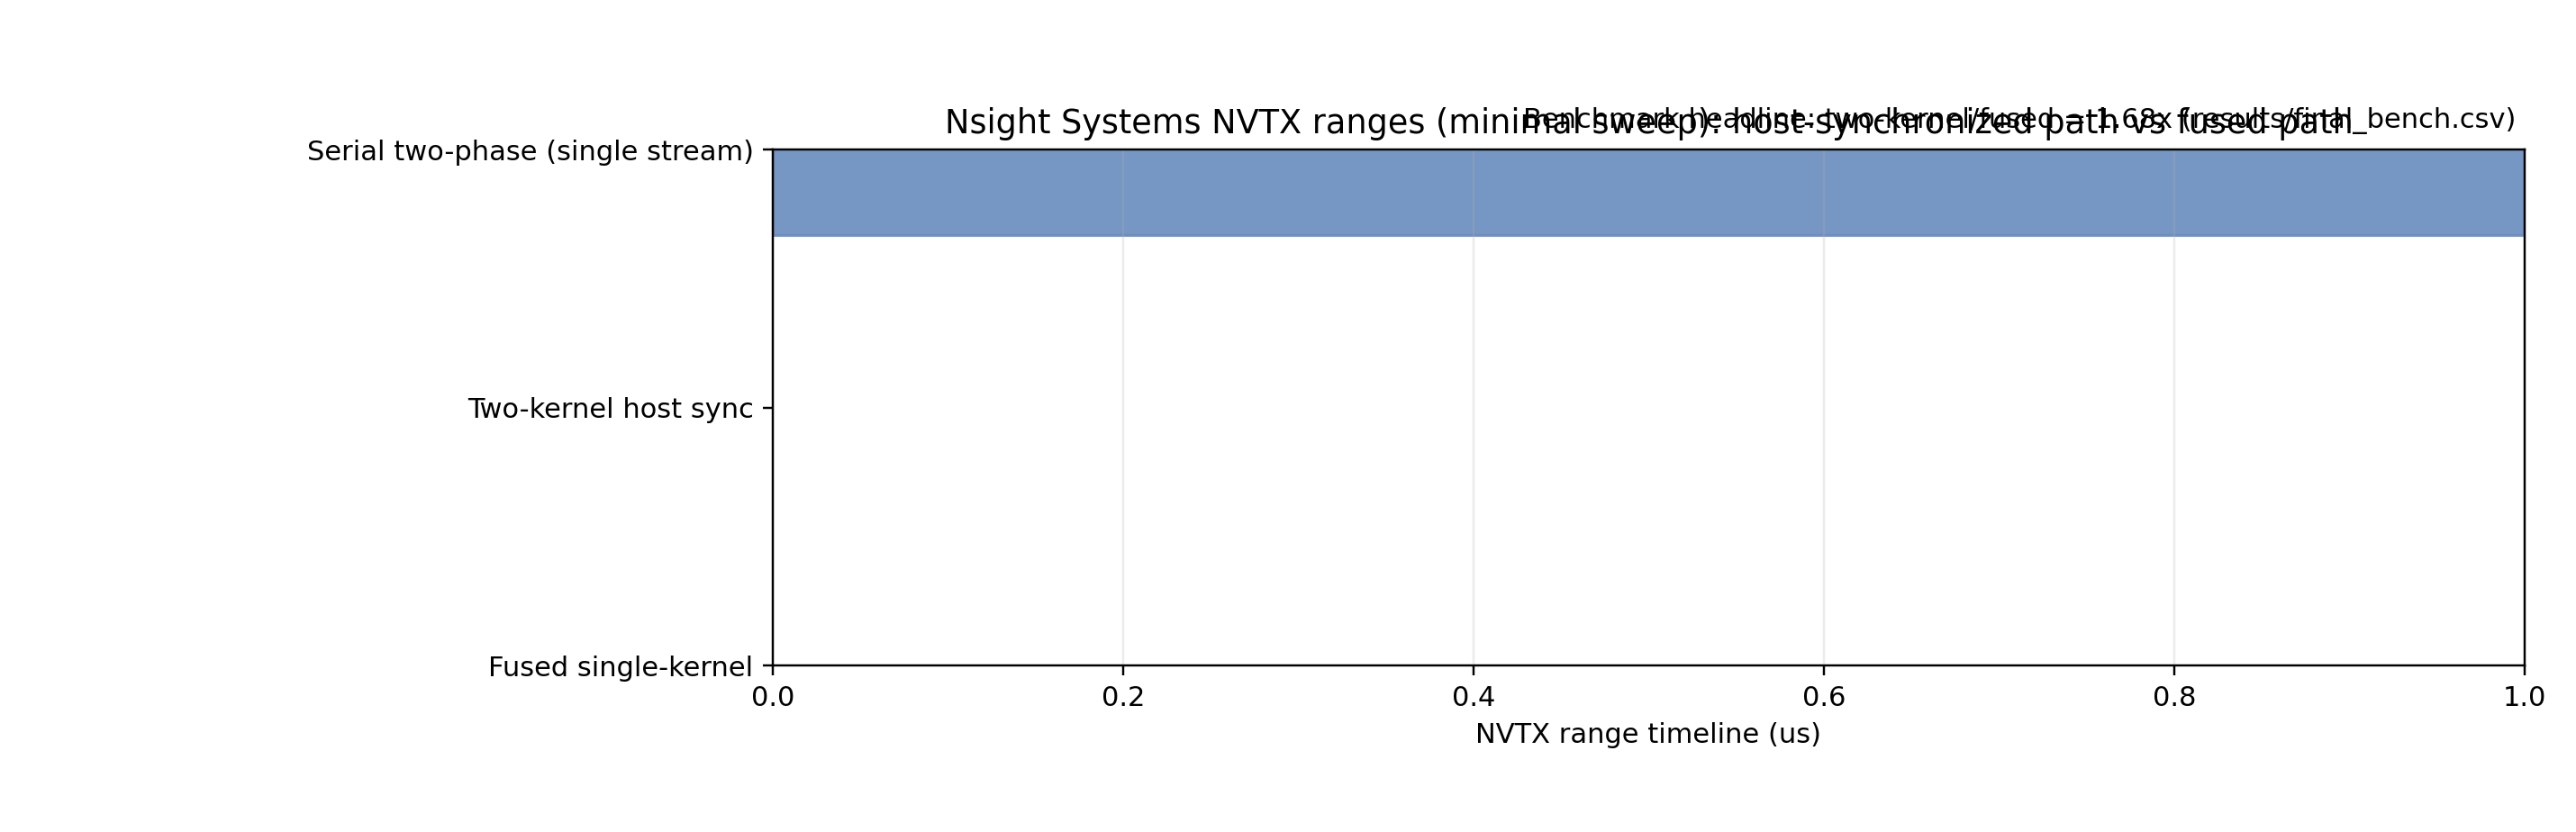
\includegraphics[width=\linewidth]{../docs/figures/overlap_nvtx_minimal.png}%
    }{%
        \framebox{\parbox[c][0.22\textwidth][c]{0.92\linewidth}{\centering
        \textit{Export \texttt{overlap\_nvtx\_minimal.png} via Nsight Systems from \texttt{capture\_nsys.sh} (see docs/figures/README.md).}}}%
    }
    \caption{Nsight Systems NVTX-range timeline from \texttt{scripts/capture\_nsys.sh -- --bench-scope minimal --skip-correctness --iters 20 --warmup 3}. The host-synchronized two-kernel region is visibly longer than the fused region. Final benchmark means in \texttt{results/final\_bench.csv}: 11.582 \(\mu s\) (two-kernel) vs 6.904 \(\mu s\) (fused), i.e. \(1.68\times\) speedup.}
\end{figure}

\end{document}
